\begin{figure}
    % WARNING: DO NOT CHANGE MANUALLY, CHANGES WILL BE OVERWRITTEN
        \ifdefined\AAAINV\else
        \newcommand\A[2]{\mathbf{A}_{#2}^{#1}}
        \newcommand\B[2]{\mathbf{B}_{#2}^{#1}}
        \newcommand\AINV[2]{(\A{#1}{#2})^{-1}}
        \newcommand\BINV[2]{(\B{#1}{#2})^{-1}}
        \newcommand\AAA[1]{\mathbf{A}^{#1}}
        \newcommand\BBB[1]{\mathbf{B}^{#1}}
        \newcommand\AAAINV[1]{(\AAA{#1})^{-1}}
        \newcommand\BBBINV[1]{(\BBB{#1})^{-1}}
        \newcommand\R{\mathbf{R}}
        \newcommand\RINV{\mathbf{R}^{-1}}
        \newcommand\M{\mathbf{M}}
        \newcommand\El{\ell'}
        \newcommand\MINV{\mathbf{M}^{-1}}
        \newcommand\Min{m_{in}}
        \newcommand\Mout{m_{out}}
        \newcommand\XOR[1]{\mathbf{X}\left[#1\right]}
        \fi
        \ifdefined\aCipher\else
        \newcommand\aCipher{\texttt{Sparkle}}
        \newcommand\FigDef[2]{\caption{#2}\label{#1}}
        \newcommand\PathFig[1]{NON_EXISTANT_PATH/#1}
        \fi
    \caption{Attack on 3.5-step \aCipher{} with whitening.
                            The green dots show known values, the purple crosses show zero differences.
                            The purple dashed areas shows the parts with the target differential transitions.}
    \label{fig:mitm3.5whit}
    \IfFileExists{\PathFig{mitm_3p5steps_whitening.pdf}}{
    \includegraphics{\PathFig{mitm_3p5steps_whitening.pdf}}
    }{
    \centering
    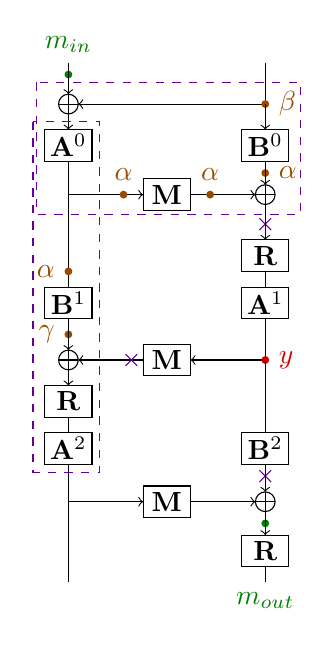
\begin{tikzpicture}[xscale=1.0,yscale=-1.0]
        \fill[green!50!black] (0.0,0.15) ellipse (0.05 and 0.05);
        \draw (0.0,0.0) node[anchor=south,green!50!black] {$\Min$};
        \draw[->] (0.0,0.0) -- (0.0,0.4);
        \draw (0.0,0.525) ellipse (0.125 and 0.125);
        \draw (0.0,0.4) -- (0.0,0.65);
        \draw (-0.125,0.525) -- (0.125,0.525);
        \draw (2.5,0.0) -- (2.5,0.525);
        \draw[->] (2.5,0.525) -- (0.125,0.525);
        \fill[orange!60!black] (2.5,0.525) ellipse (0.05 and 0.05);
        \draw (2.55,0.525) node[anchor=west,orange!60!black] {$\boldsymbol{\beta}$};
        \draw[->] (0.0,0.65) -- (0.0,0.85);
        \draw (-0.3,0.85) rectangle (0.3,1.25) node[pos=0.5] {$\AAA{0}$};
        \draw[->] (2.5,0.525) -- (2.5,0.85);
        \draw (2.2,0.85) rectangle (2.8,1.25) node[pos=0.5] {$\BBB{0}$};
        \fill[orange!60!black] (2.5,1.4) ellipse (0.05 and 0.05);
        \draw (2.55,1.4) node[anchor=west,orange!60!black] {$\boldsymbol{\alpha}$};
        \draw (0.0,1.25) -- (0.0,1.675);
        \draw[->] (2.5,1.25) -- (2.5,1.55);
        \draw (2.5,1.675) ellipse (0.125 and 0.125);
        \draw (2.5,1.55) -- (2.5,1.8);
        \draw (2.375,1.675) -- (2.625,1.675);
        \draw[->] (0.0,1.675) -- (0.95,1.675);
        \draw (0.95,1.475) rectangle (1.55,1.875) node[pos=0.5] {$\M$};
        \draw[->] (1.55,1.675) -- (2.375,1.675);
        \fill[orange!60!black] (0.7,1.675) ellipse (0.05 and 0.05);
        \draw (0.7,1.625) node[anchor=south,orange!60!black] {$\boldsymbol{\alpha}$};
        \fill[orange!60!black] (1.8,1.675) ellipse (0.05 and 0.05);
        \draw (1.8,1.625) node[anchor=south,orange!60!black] {$\boldsymbol{\alpha}$};
        \draw[red!40!blue] (2.425,1.975) -- (2.575,2.125);
        \draw[red!40!blue] (2.425,2.125) -- (2.575,1.975);
        \draw[->] (2.5,1.8) -- (2.5,2.25);
        \draw (2.2,2.25) rectangle (2.8,2.65) node[pos=0.5] {$\R$};
        \draw (0.0,1.675) -- (0.0,2.85);
        \draw (2.5,2.65) -- (2.5,2.85);
        \draw (-0.3,2.85) rectangle (0.3,3.25) node[pos=0.5] {$\BBB{1}$};
        \draw (2.2,2.85) rectangle (2.8,3.25) node[pos=0.5] {$\AAA{1}$};
        \fill[orange!60!black] (0.0,2.65) ellipse (0.05 and 0.05);
        \draw (-0.05,2.65) node[anchor=east,orange!60!black] {$\boldsymbol{\alpha}$};
        \fill[orange!60!black] (0.0,3.45) ellipse (0.05 and 0.05);
        \draw (-0.05,3.45) node[anchor=east,orange!60!black] {$\boldsymbol{\gamma}$};
        \draw[->] (0.0,3.25) -- (0.0,3.65);
        \draw (0.0,3.775) ellipse (0.125 and 0.125);
        \draw (0.0,3.65) -- (0.0,3.9);
        \draw (-0.125,3.775) -- (0.125,3.775);
        \draw (2.5,3.25) -- (2.5,3.775);
        \draw[->] (2.5,3.775) -- (1.55,3.775);
        \draw (0.95,3.575) rectangle (1.55,3.975) node[pos=0.5] {$\M$};
        \draw[->] (0.95,3.775) -- (0.125,3.775);
        \draw[->] (0.0,3.9) -- (0.0,4.1);
        \draw (-0.3,4.1) rectangle (0.3,4.5) node[pos=0.5] {$\R$};
        \fill[red!80!black] (2.5,3.775) ellipse (0.05 and 0.05);
        \draw (2.55,3.775) node[anchor=west,red!80!black] {$y$};
        \draw[red!40!blue] (0.725,3.7) -- (0.875,3.85);
        \draw[red!40!blue] (0.725,3.85) -- (0.875,3.7);
        \draw (0.0,4.5) -- (0.0,4.7);
        \draw (2.5,3.775) -- (2.5,4.7);
        \draw (-0.3,4.7) rectangle (0.3,5.1) node[pos=0.5] {$\AAA{2}$};
        \draw (2.2,4.7) rectangle (2.8,5.1) node[pos=0.5] {$\BBB{2}$};
        \draw[red!40!blue] (2.425,5.175) -- (2.575,5.325);
        \draw[red!40!blue] (2.425,5.325) -- (2.575,5.175);
        \draw (0.0,5.1) -- (0.0,5.575);
        \draw[->] (2.5,5.1) -- (2.5,5.45);
        \draw (2.5,5.575) ellipse (0.125 and 0.125);
        \draw (2.5,5.45) -- (2.5,5.7);
        \draw (2.375,5.575) -- (2.625,5.575);
        \draw[->] (0.0,5.575) -- (0.95,5.575);
        \draw (0.95,5.375) rectangle (1.55,5.775) node[pos=0.5] {$\M$};
        \draw[->] (1.55,5.575) -- (2.375,5.575);
        \fill[green!50!black] (2.5,5.85) ellipse (0.05 and 0.05);
        \draw[->] (2.5,5.7) -- (2.5,6.0);
        \draw (2.2,6.0) rectangle (2.8,6.4) node[pos=0.5] {$\R$};
        \draw (0.0,5.575) -- (0.0,6.6);
        \draw (2.5,6.4) -- (2.5,6.6);
        \draw[dashed,red!40!blue] (-0.45,0.75) rectangle (0.4,5.2);
        \draw[dashed,red!40!blue] (-0.4,0.25) rectangle (2.95,1.925);
        \draw (2.5,6.6) node[anchor=north,green!50!black] {$\Mout$};
    \end{tikzpicture}
    }
\end{figure}
